\documentclass[12pt,a4paper]{article} % this tells LaTeX to make the
\usepackage[utf8]{inputenc} 
\usepackage[boxed]{algorithm2e} 
\usepackage{cite}
\usepackage{color}
\usepackage{listings}
\usepackage{graphicx, subfigure}
\lstset{ %
language=C++, % choose the language of the code
basicstyle=\footnotesize, % the size of the fonts that are used for the code
numbers=left, % where to put the line-numbers
numberstyle=\footnotesize, % the size of the fonts that are used for the line-numbers
stepnumber=0, % the step between two line-numbers. If it is 1 each line will be numbered
numbersep=5pt, % how far the line-numbers are from the code
backgroundcolor=\color{white}, % choose the background color. You must add \usepackage{color}
showspaces=false, % show spaces adding particular underscores
showstringspaces=false, % underline spaces within strings
showtabs=false, % show tabs within strings adding particular underscores
frame=single, % adds a frame around the code
tabsize=2, % sets default tabsize to 2 spaces
captionpos=b, % sets the caption-position to bottom
breaklines=true, % sets automatic line breaking
breakatwhitespace=false, % sets if automatic breaks should only happen at whitespace
escapeinside={\%}{)} % if you want to add a comment within your code
}
\usepackage{amsmath} % a very handy maths typesetting
% package from the
% American Mathematical Society
\usepackage{graphicx} % the standard
% report on a4 paper, at 12pt
% (nice and easy to read) and
% to use the report class file
% (a file that defines how the
% report should look when
% finished so that you can
% concentrate on content).
% the bit between the \documentclass statement and the
% \begin{document} statement is called the ``preamble''
% you may have noticed that comments are denoted by a % sign
\title{Solving Sudoku with MATLAB and GUIDE} % put in a title (if
% you want a title page
\author{Raluca Marinescu, Andrea Garcia, Ivan Castro, Eduard Enoiu} % put in the author
% (if you want a title page)
\begin{document} % start of the document
\maketitle % makes the title page
\begin{abstract}
\end{abstract}
\section{Introduction}
\subsection{The Problem}
\subsection{Related Works}
Sudoku puzzles can be viewed as a interesting problem for different fields of mathematics, computer science, artificial intelligence, physics, and others. There are many researchers from these fields who have proposed algorithms to solve puzzles in many different ways. 
\newline
\\ In \cite{jones2008construction} the authors proposes a search based solution in order to solve Sudoku puzzles by using some heuristic in a modified steepest hill ascent. Some researchers, as found here \cite{mantere2007solving}, are suggesting the design of a genetic algorithm by representing the puzzle as a block of chromosomes, more precise as an array of 81 integers. Any crossover appears between the 3x3 grids and any mutations occur only inside the 3x3 grids. From the experiments done in \cite{mantere2007solving} the algorithm based on genetic algorithms performs well though is does not solve all cases. Geem in \cite{geem2008harmony} proposes a model for a Sudoku solver based on harmony search that mimics the characteristics of a musician. As mentioned in \cite{green2009survey} the performance of the algorithms is not that good and it solves puzzles in less than 40 seconds and in less than 300 iterations. Santos-Garcia and Palomino suggests here \cite{santos2007solving} a method for solving Sudoku puzzles using simple logic with rewriting rules to mimic human intelligence. This method works but, as the author admits, it is not performing well when compared with other techniques. Others like \cite{yue2006sudoku} are suggesting neural networks by modelling an energy driven quantum neuron (Q'tron) neural network to solve the Sudoku puzzles. 
\newline
\\ In \cite{bartlett2006integer}, Barlett and Langville proposes a solution based on binary integer linear programming (BILP). To formulate in a simple way the method we can say that it uses binary variables to pick a digit for a cell in Sudoku puzzle. The model in \cite{bartlett2006integer} is solved in MATLAB and it works very fast (16 sec. per second).
\newline
\\ In \cite{norvigsolving}, Russell Norvig is suggesting a solution based on backtracking. The algorithm is a combination of constraint propagation and direct search by assigning a value to a square on the grid and then propagating these constraints to other squares.
\newline
\\ We have decided to solve the puzzles using backtracking as in \cite{norvigsolving} because of the simplicity and performance mentioned by Norvig. We will present in the next section our own algorithm using recursive backtracking and constraint propagation.
\section{Implementation}
\subsection{GUI Design}
\subsection{An Algorithm for Solving Sudoku Puzzles}
The algorithm was implemented in MATLAB using direct search and constraint propagation. This constraint propagation was implemented in such a manner that: 
\begin{itemize}
\item When a value is assigned to a square that same value cannot be used as a possible assignment in all related squares
\item If a square has only one single value for possible assignment, that value is immediately assigned.
\end{itemize}
Our MATLAB program has only 5 steps:
\begin{itemize}
\item Find all the possible values for all empty cells
\item Assign a value to a square on the grid
\item Propagate constraints to other square
\item If all the cells have more than one possible value we fill in a tentative value for one cell
\end{itemize}
This algorithm, though it is simplistic, it should by the nature of the algorithm class perform in a fairly way. This algorithm performs in up left to right and up to down fashion.
\newline
\\ To see how our program works, we will use a simpler 4-by-4 grid with 2-by-2 blocks. As mentioned in \cite{crook2009pencil} these kinds of puzzles are called Shidoku ("Shi" means "four" in Japanese). 
\begin{figure}[ht!]
\label{fig:subfigures}
\begin{center}
%
\subfigure[A Shidoku puzzle]{%
\label{fig:first}
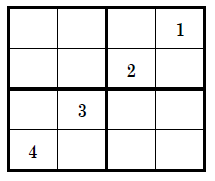
\includegraphics[width=0.4\textwidth]{pictures/1.png}
}%
\subfigure[The possible candidates for all squares]{%
\label{fig:second}
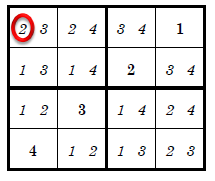
\includegraphics[width=0.4\textwidth]{pictures/2.png}
}\\ % ------- End of the first row ----------------------%
\subfigure[Inserting value 2 and constraint propagation]{%
\label{fig:third}
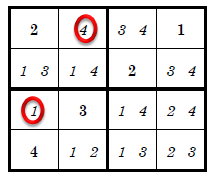
\includegraphics[width=0.4\textwidth]{pictures/3.png}
}%
\subfigure[Constraint propagation]{%
\label{fig:fourth}
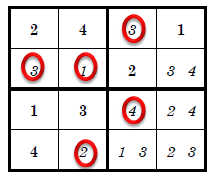
\includegraphics[width=0.4\textwidth]{pictures/4.png}
}\\ % ------- End of the second row ----------------------%
\subfigure[Insert the remaining values to complete the puzzle]{%
\label{fig:fifth}
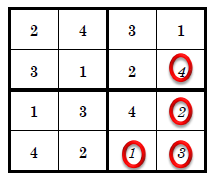
\includegraphics[width=0.4\textwidth]{pictures/5.png}
}%
\subfigure[The puzzle completed]{%
\label{fig:sixth}
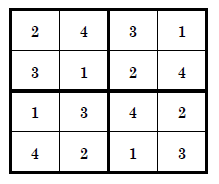
\includegraphics[width=0.4\textwidth]{pictures/6.png}
}
\end{center}
\caption{%
Algorithm Exemplification by using a simple example
}%
\end{figure}
Figure 1(a) shows a Shidoku puzzle. Figure 1(b) through 1(f) shows how we get to a solution by using our algorithm. In Figure 1(b), the possible assignment, are represented as smaller digits. For example in Figure 1(b) line 1, row 1, we have two possible values to choose from. If a cell contains only one candidate is filled immediately.
\newline
\\ In the next section we are presenting some testing results under different puzzles and we will describe how our MATLAB behaves to various situations. 
\section{Experimental Results}
\section{Conclusions}
\bibliography{mybib}{}
\bibliographystyle{plain}
\end{document}

